\chapter{Arhitektura i dizajn sustava}
		
		Arhitekturu našeg sustava možemo podijeliti na tri podsustava:	
		\begin{itemize}
		\item 	\textit{Web preglednik}
		\item 	\textit{Baza podataka}
		\item 	\textit{Web poslužitelj}		
		\end{itemize}
		
		\begin{figure}[H]
			\centering
			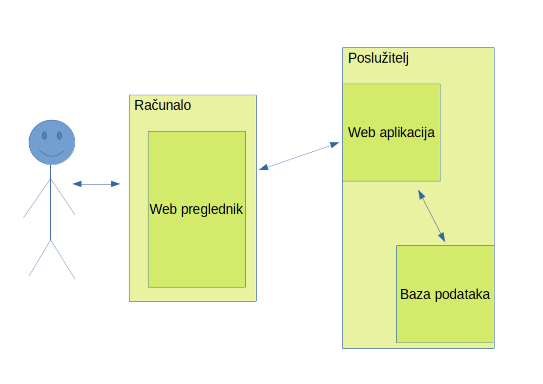
\includegraphics[width=\textwidth, scale=2.0]{slike/arhitektura.png}
			\caption{Arhitektura sustava}
			\label{fig:arhitektura}
		\end{figure}
\eject
	
	
	
	\underbar{ \textit{Web preglednik} }{je program koji korisniku omogućuje pregled web-stranica i multi-medijalnih sadržaja vezanih uz njih. Korisnik putem web preglednika šalje zahtjeve na obradu poslužitelju.}

	\underbar{ \textit{Baza podataka}}{ je zbirka zapisa pohranjenih u računalu na sustavan način, tako da joj se računalni program može obratiti prilikom odgovaranja na problem. Web poslužitelj komunicira s bazom podataka te povlači potrebne zapise iz nje.}
	
	\underbar{ \textit{Web poslužitelj}}{ je srce našeg sustava. Njegova zadaća je komunikacija klijenta s aplikacijom te bazom podataka. Pri komunikaciji koristi HTTP protokol.Korisnik i aplikacija razmjenjuju HTTP zahtjeve (eng. HTTP request) i HTTP odgovore (HTTP response). Radi jednostavnosti, baza podataka je također smještena na poslužitelju.}\\
	Korisnik kroz grafičko sučelje, odnosno frontend, šalje zahtjeve na REST pristupne točke backenda. Tada backend procesuira zahtjev i ako je potrebno komunicira s bazom podataka. Nakon konstrukcije, backend šalje odgovor frontendu u obliku JSON objekta, a frontend procesuira odgovor i promjene prikazuje korisniku u obliku HTML stranice.
\eject
	Programski jezik kojeg smo odabrali za izradu naše web aplikacije je Java zajedno s Spring radnim okvirom te programski jezik JavaScript u sklopu React-a. Odabrana razvojna okruženja su Eclipse i IntelliJ IDEA. Za aplikaciju je odabrana višeslojna arhitektura temeljena na \textbf{MVC} (Model - View - Controller) arhitekturnom stilu te uslužnoj arhitekturi. Podjela slojeva možemo napraviti na idući način:
	\begin{figure}[H]
			\centering
			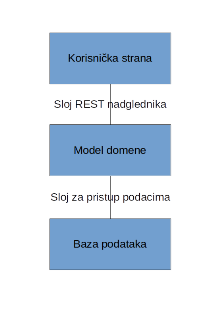
\includegraphics[scale=0.9]{slike/arhitektura2.png}
			\caption{Podjela slojeva}
			\label{fig:slojevi}
		\end{figure}
	\begin{itemize}
		\item 	\textit{sloj korisničke strane} - korisničko sučelje
		\item 	\textit{sloj nadglednika} - REST nadglednici
		\item 	\textit{sloj domene}	- model podataka iz domene primjene
		\item 	\textit{sloj za pristup podacima} - posrednik između sloja domene i baze podataka
		\item 	\textit{sloj baze podataka} - pohrana podataka	
		\end{itemize}

\eject	{Ovakva arhitektura odabrana je zbog poželjnih svojstava MVC arhitekturnog stila i višeslojne arhitekture: razvoj pojedinih slojeva je jednostavniji i u velikom stupnju nezavisan od razvoja drugih slojeva. Također komunikacija frontenda i backenda ostvarena je primjenom REST arhitekturnog stila. Zbog toga su i frontend i backend neovisni o jeziku implementacije, što potiče ponovnu uporabu. }
	
	 {Model-View-Controller se sastoji od:}
	\begin{itemize}
		\item 	\textbf{Model} {je centralni dio aplikacije, koja obuhvaća promjenljivu (dinamičku) strukturu podataka, direktno upravljanje podacima, logikom i pravilima aplikacije}
		\item 	\textbf{View}{ je bilo koji izlazni prikaz podataka u korisničkom okruženju, pri čemu se isti podaci mogu prikazati na više načina}
		\item 	\textbf{Controller} {ulazne podatke pretvara u komande koje upravljaju modelom ili prikazom podataka u korisničkom okruženju}
	\end{itemize}
	
		\begin{figure}[H]
			\centering
			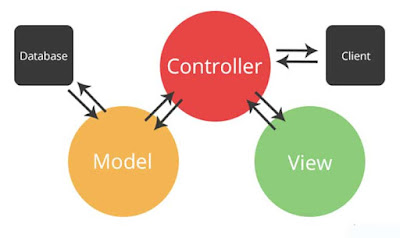
\includegraphics[width=100mm, scale=0.1]{slike/MVC.jpeg}
			\caption{MVC model}
			\label{fig:arhitektura}
		\end{figure}
\eject

		

				
		\section{Baza podataka}
			
			
			
		Za potrebe našeg sustava koristit ćemo relacijsku bazu podataka koja svojom strukturom olakšava modeliranje stvarnog svijeta. Gradivna jedinka baze je relacija, odnosno tablica koja je definirana svojim imenom i skupom atributa. Zadaća baze podataka je brza i jednostavna pohrana, izmjena i dohvat podataka za daljnju obradu.
Baza podataka ove aplikacije sastoji se od sljedećih entiteta: 
\begin{itemize}
		\item korisnikAplikacije
		\item uloge
		\item pokusajDoniranja
		\item krvnaVrsta
		\item potrosnjaKrvi
		\item zdravstveniPodaci
		\item doniranjeZdravljeOdgovori
		
	\end{itemize}

		\eject
			\subsection{Opis tablica}
			

				\textbf{korisnikAplikacije \textit{•}}
				 Ovaj entitet predstavlja sve korisnike aplikacije (admin, djelatnik, donor) i diferencira ih pomoću ulogaId što je referenca na tablicu uloga.Za admina i djelatnika postoje atributi : ime, prezime, oib, email dok su ostale vrijednosti null. Kod stvaranja atributa trajnoOdbijanjeDarivanja je false, a razlogOdbijanja je null ,ako se korisniku odbije darivanje zauvijek onda se ti atributi mijenjaju. One-to-many veza s pokusajDoniranja preko korisnikID dvaput, One-to-many veza s potrosnjaKrvi preko korisnikId, many-to-one veza s uloge preko ulogaId i many-to-one veza s krvnaVrsta preko krvId.

				
				\begin{longtblr}[
					label=none,
					entry=none
					]{
						width = \textwidth,
						colspec={|X[15,l]|X[6, l]|X[20, l]|}, 
						rowhead = 1,
					} %definicija širine tablice, širine stupaca, poravnanje i broja redaka naslova tablice
					\hline \multicolumn{3}{|c|}{\textbf{korisnikAplikacije}}	 \\ \hline[3pt]				
					\SetCell{LightGreen}korisnikId & VARCHAR & id pomoću kojeg se korisnik prijavljuje u sustav (jednako donorId za donore)\\ \hline
					lozinka	& VARCHAR &  hash korisničke lozinke 	\\ \hline 
					ime & VARCHAR	&  ime korisnika		\\ \hline 
					prezime & VARCHAR	& prezime korisnika	\\ \hline 
					mjestoRodenja & VARCHAR & mjesto rođenja (nullable) \\ \hline
					oib & VARCHAR & oib korisnika \\ \hline
					adresaStanovanja & VARCHAR & adresa stanovanja (nullable) \\ \hline
					mjestoZaposlenja & VARCHAR & firma u kojoj je korisnik zaposlen (nullable) \\ \hline
					email & VARCHAR & email na koji korisniku dolaze korisne informacije (nullable) \\ \hline 
					brojMobitelaPrivatni & VARCHAR	&  privatni broj korisnika	(nullable)	\\ \hline
					brojMobitelaPoslovni & VARCHAR	&  broj na koji korisniku dolaze korisne infromacije poslovni(nullable)\\ \hline
                     datumRodenja & DATE &  datum rođenja	\\ \hline
                     \SetCell{LightBlue}krvId & INT & vrsta krvi donora \\ \hline
                     trajnoOdbijenoDarivanje & BOOLEAN &  true ako je korisniku zabranjeno trajno darivanje, false ako nije \\ \hline
					 \SetCell{LightBlue}ulogaId & BIGINT &  oznaka uloge korisnika \\ \hline 
					aktivacijskiKljuc & VARCHAR(10) & aktivacijski ključ koji služi za aktivaciju računa \\
\hline		
					\end{longtblr}
				
				\textbf{uloge \textit{•}}
				entitet koji sadrži dva atributa, id za oznaku rednog broja uloge i ulogaName za ime 						uloge
				One-to-many veza s korisnikAplikacije preko ulogaId.
				\begin{longtblr}[
					label=none,
					entry=none
					]{
						width = \textwidth,
						colspec={|X[6,l]|X[6, l]|X[20, l]|}, 
						rowhead = 1,
					} %definicija širine tablice, širine stupaca, poravnanje i broja redaka naslova tablice
					\hline \multicolumn{3}{|c|}{\textbf{Uloge}}	 \\ \hline[3pt]
					\SetCell{LightGreen}ulogaId & BIGINT & označava id uloge \\ \hline
					ulogaName	& VARCHAR & naziv uloge	\\ \hline 
					
				\end{longtblr}
	\eject
				\textbf{pokusajDonacije\textit{•}}
				-entitet koji predstavlja pokušaj doniranja, sadrži podatke o datumu, mjestu, darivatelju, djelatniku, uspješnosti i razlogu odbijanja ako je uspješnost false.
				Many-to-one veza preko korisnikIdDjelatnika s korisnikAplikacije , Many-to-one veza preko korisnikIdDonora s korisnikAplikacije, one-to-many veza s doniranjeZdravljeOdgovori reko brDoniranja.
				
				\begin{longtblr}[
					label=none,
					entry=none
					]{
						width = \textwidth,
						colspec={|X[15,l]|X[6, l]|X[20, l]|}, 
						rowhead = 1,
					} %definicija širine tablice, širine stupaca, poravnanje i broja redaka naslova tablice
					\hline \multicolumn{3}{|c|}{\textbf{pokusajDonacije}}	 \\ \hline[3pt]
					\SetCell{LightGreen}brDoniranja & BIGINT & redni broj donacije\\ \hline
					datum & DATE & datum donacije \\ \hline
					mjestoDarivanja	& VARCHAR & opisno mjesto donacije	\\ \hline 
					\SetCell{LightBlue}korisnikIdDjelatnika & VARCHAR & identifikator djelatnika \\ \hline
					\SetCell{LightBlue}korisnikId & VARCHAR & identifikator donora \\ \hline

					uspjeh	& BOOLEAN & oznaka uspješnosti darivanja  	\\ \hline 			
					
				\end{longtblr}
				
				\textbf{krvnaVrsta\textit{•}}
				
				- entitet čuva podatke o zalihi i predviđenim gornjim i donjim granicama za sve krvne grupe.  one-to-many veza s potrosnjaKrvi preko krvId i one-to-many veza s korisnikAplikacije preko krvId.
				\begin{longtblr}[
					label=none,
					entry=none
					]{
						width = \textwidth,
						colspec={|X[15,l]|X[6, l]|X[20, l]|}, 
						rowhead = 1,
					} %definicija širine tablice, širine stupaca, poravnanje i broja redaka naslova tablice
					\hline \multicolumn{3}{|c|}{\textbf{krvnaVrsta}}	 \\ \hline[3pt]
					\SetCell{LightGreen}krvId & SERIAL & identifikator krvne grupe \\ \hline
					imeKrvneGrupe & VARCHAR & naziv krvne grupe \\ \hline
					gornjaGranica & INT & gornja granica dopuštene količine krvi u jedinicama\\ \hline

					donjaGranica	& INT & donja granica dopuštene količine krvi u jedinicama  	\\ \hline 
					trenutnaZaliha	& INT &  trenutna zaliha konkretne krvne grupe u jedinicama 	\\ \hline 
					
					
				\end{longtblr}
\eject			
				
				\textbf{potrosnjaKrvi\textit{•}}
				
				entitet koji prati isporuke krvi . 
				Many-to-one veza s korisnikAplikacije preko korisnikIdDjelatnika i Many-to-one veza s krvnaVrsta preko krvId.

				\begin{longtblr}[
					label=none,
					entry=none
					]{
						width = \textwidth,
						colspec={|X[15,l]|X[6, l]|X[20, l]|}, 
						rowhead = 1,
					} %definicija širine tablice, širine stupaca, poravnanje i broja redaka naslova tablice
					\hline \multicolumn{3}{|c|}{\textbf{potrosnjaKrvi}}	 \\ \hline[3pt]
					\SetCell{LightGreen} idPotrosnje & SERIAL & redni broj isporuke krvi \\ \hline
					timestampPotrosnje & TIMESTAMP & timestamp potrošnje \\ \hline
					\SetCell{LightBlue}krvId & INT & id krvne grupe \\ \hline
					količinaJedinica & INT &  broj jedinica koje su se potrošili \\ \hline 
					
					\SetCell{LightBlue}korisnikIdDjelatnika & VARCHAR &  identifikator djelatnika koji je inicirao slanje krvi bolnici	\\ \hline 
					lokacijaPotrosnje & VARCHAR & opisna lokacija kamo ide isporuka krvi \\ \hline
					
				\end{longtblr}
				
				\textbf{zdravstveniPodaci\textit{•}}
				
				entitet koji sprema sve moguće zdravstvene podatke koji se pitaju korisnika u upitniku. Oni sadrže svoj id, koji se sam generira u tablici, opis zdravstvenog podatka i težinu kriterija odnosno, 0 ako se na temelju toga podatka trajno odbija darivanje i 1 ako se privremeno odbija, inače null.
				One-to-many veza s doniranjeZdravljeOdgovori preko idZdravstvenih.
				\begin{longtblr}[
					label=none,
					entry=none
					]{
						width = \textwidth,
						colspec={|X[10,l]|X[6, l]|X[20, l]|}, 
						rowhead = 1,
					} %definicija širine tablice, širine stupaca, poravnanje i broja redaka naslova tablice
					\hline \multicolumn{3}{|c|}{\textbf{zdravstveniPodaci}}	 \\ \hline[3pt]
					\SetCell{LightGreen}idZdravstvenih & SERIAL & id zdravstvenog podatka \\ \hline
					zdravstveniPodatak & VARCHAR & opis zdravstvenog podatka koji se ispituje
					npr. osoba teži manje od 55 kg \\ \hline
					tezinaKriterija 	& INT &  tezina kriterija ( 0 za trajno, 1 za privremeno) 	\\ \hline 

					
				\end{longtblr}
\eject				
				\textbf{doniranjeZdravljeOdgovori\textit{•}}
				
				entitet koji služi kao spremište odgovora korisnika koji su došli donirati krv.
				Many-to-one veza s zdravstveniPodaci preko idZdravstvenih. Many-to-one veza s pokusajDoniranja preko brDoniranja.
				\begin{longtblr}[
					label=none,
					entry=none
					]{
						width = \textwidth,
						colspec={|X[10,l]|X[6, l]|X[20, l]|}, 
						rowhead = 1,
					} %definicija širine tablice, širine stupaca, poravnanje i broja redaka naslova tablice
					\hline \multicolumn{3}{|c|}{\textbf{doniranjeZdravljeOdgovori}}	 \\ \hline[3pt]
					\SetCell{LightGreen} brDoniranja & INT & brDoniranja iz tablice pokusajDoniranja \\ \hline
					\SetCell{LightGreen} idZdravstvenih & INT &  idZdravstvenih iz tablice zdravstveni podaci \\ \hline
					odgovorDonora & BOOLEAN & odgovor donora na zdravstveni podatak pod idZdravstvenih\\ \hline
					
				\end{longtblr}
			
			\subsection{Dijagram baze podataka}
				\begin{figure}[H]
	\centering
	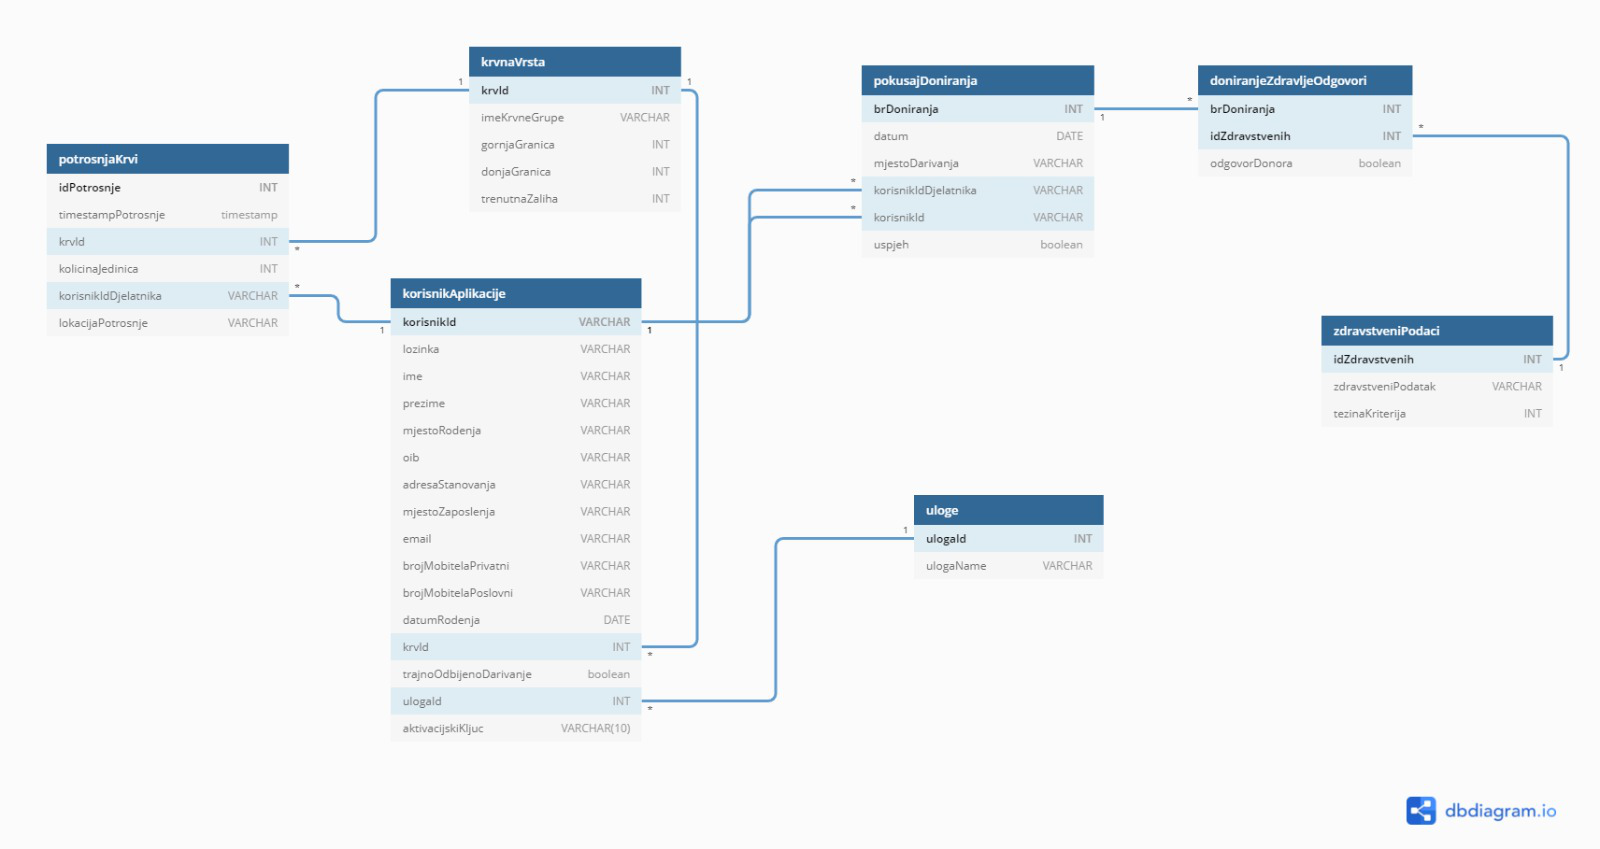
\includegraphics[width=\textwidth, scale=2.0]{dijagrami/relShema.png}
	\caption{relacijski model baze podataka}
	\label{fig:dijagram_baze}
\end{figure}
			\eject
			
		\section{Dijagram razreda}
		
<<<<<<< HEAD
	Dijagram razreda pokazuje odnose između različitih objekata, te njihove atribute i operacije kojima vladaju. Na slikama 4.5., 4.6, 4.7. prikazani su razredi koji pripadaju \textit{backend} dijelu naše arhitekture. Radi jednostavnosti, dijagram razreda je podijeljen u više slika, no bez obzira na to, prikazani razredi na neki način komuniciraju.
	Na idućoj slici prikazan je model podataka kojima backend rukuje. Korisnik aplikacije (administartor, djelatnik banke, donor) modeliran je razredom \textit{User}. Razred \textit{Blood} modelira krvne grupe. Razred \textit{Consumption} modelira potrošnju krvi. Razred \textit{Donation} modelira pokušaj donacije krvi, dok razred \textit{Role} modelira 3 moguće uloge u aplikaciji. Razred HealthData modelira zdravstvena pitanja, a HealthDataAnswered modelira odgovore na određena zdravstvena pitanja. Također navedene su enumeracije za nazive krvnih grupa i nazive uloga.
=======
	Dijagram razreda pokazuje odnose između različitih objekata, te njihove atribute i operacije kojima vladaju. Na slikama 4.5., 4.6, 4.7., 4.8 prikazani su razredi koji pripadaju \textit{backend} dijelu naše arhitekture. Radi jednostavnosti, dijagram razreda je podijeljen u više slika, no bez obzira na to, prikazani razredi na neki način komuniciraju.
	Na idućoj slici prikazan je model podataka kojima backend rukuje. Korisnik aplikacije (administartor, djelatnik banke, donor) modeliran je razredom \textit{User}. Razred \textit{Blood} modelira krvne grupe. Razred \textit{Consumption} modelira potrošnju krvi. Razred \textit{Donation} modelira pokušaj donacije krvi, dok razred \textit{Role} modelira 3 moguće uloge u aplikaciji. Razredi \textit{HealthData}, \textit{HealthDataAnswered} i \textit{HealthDataAnsweredId} modeliraju zdravstvene podatke potrebne za donacije. Također navedene su enumeracije za nazive krvnih grupa i nazive uloga.
>>>>>>> devdoc
\begin{figure}[H]
	\centering
	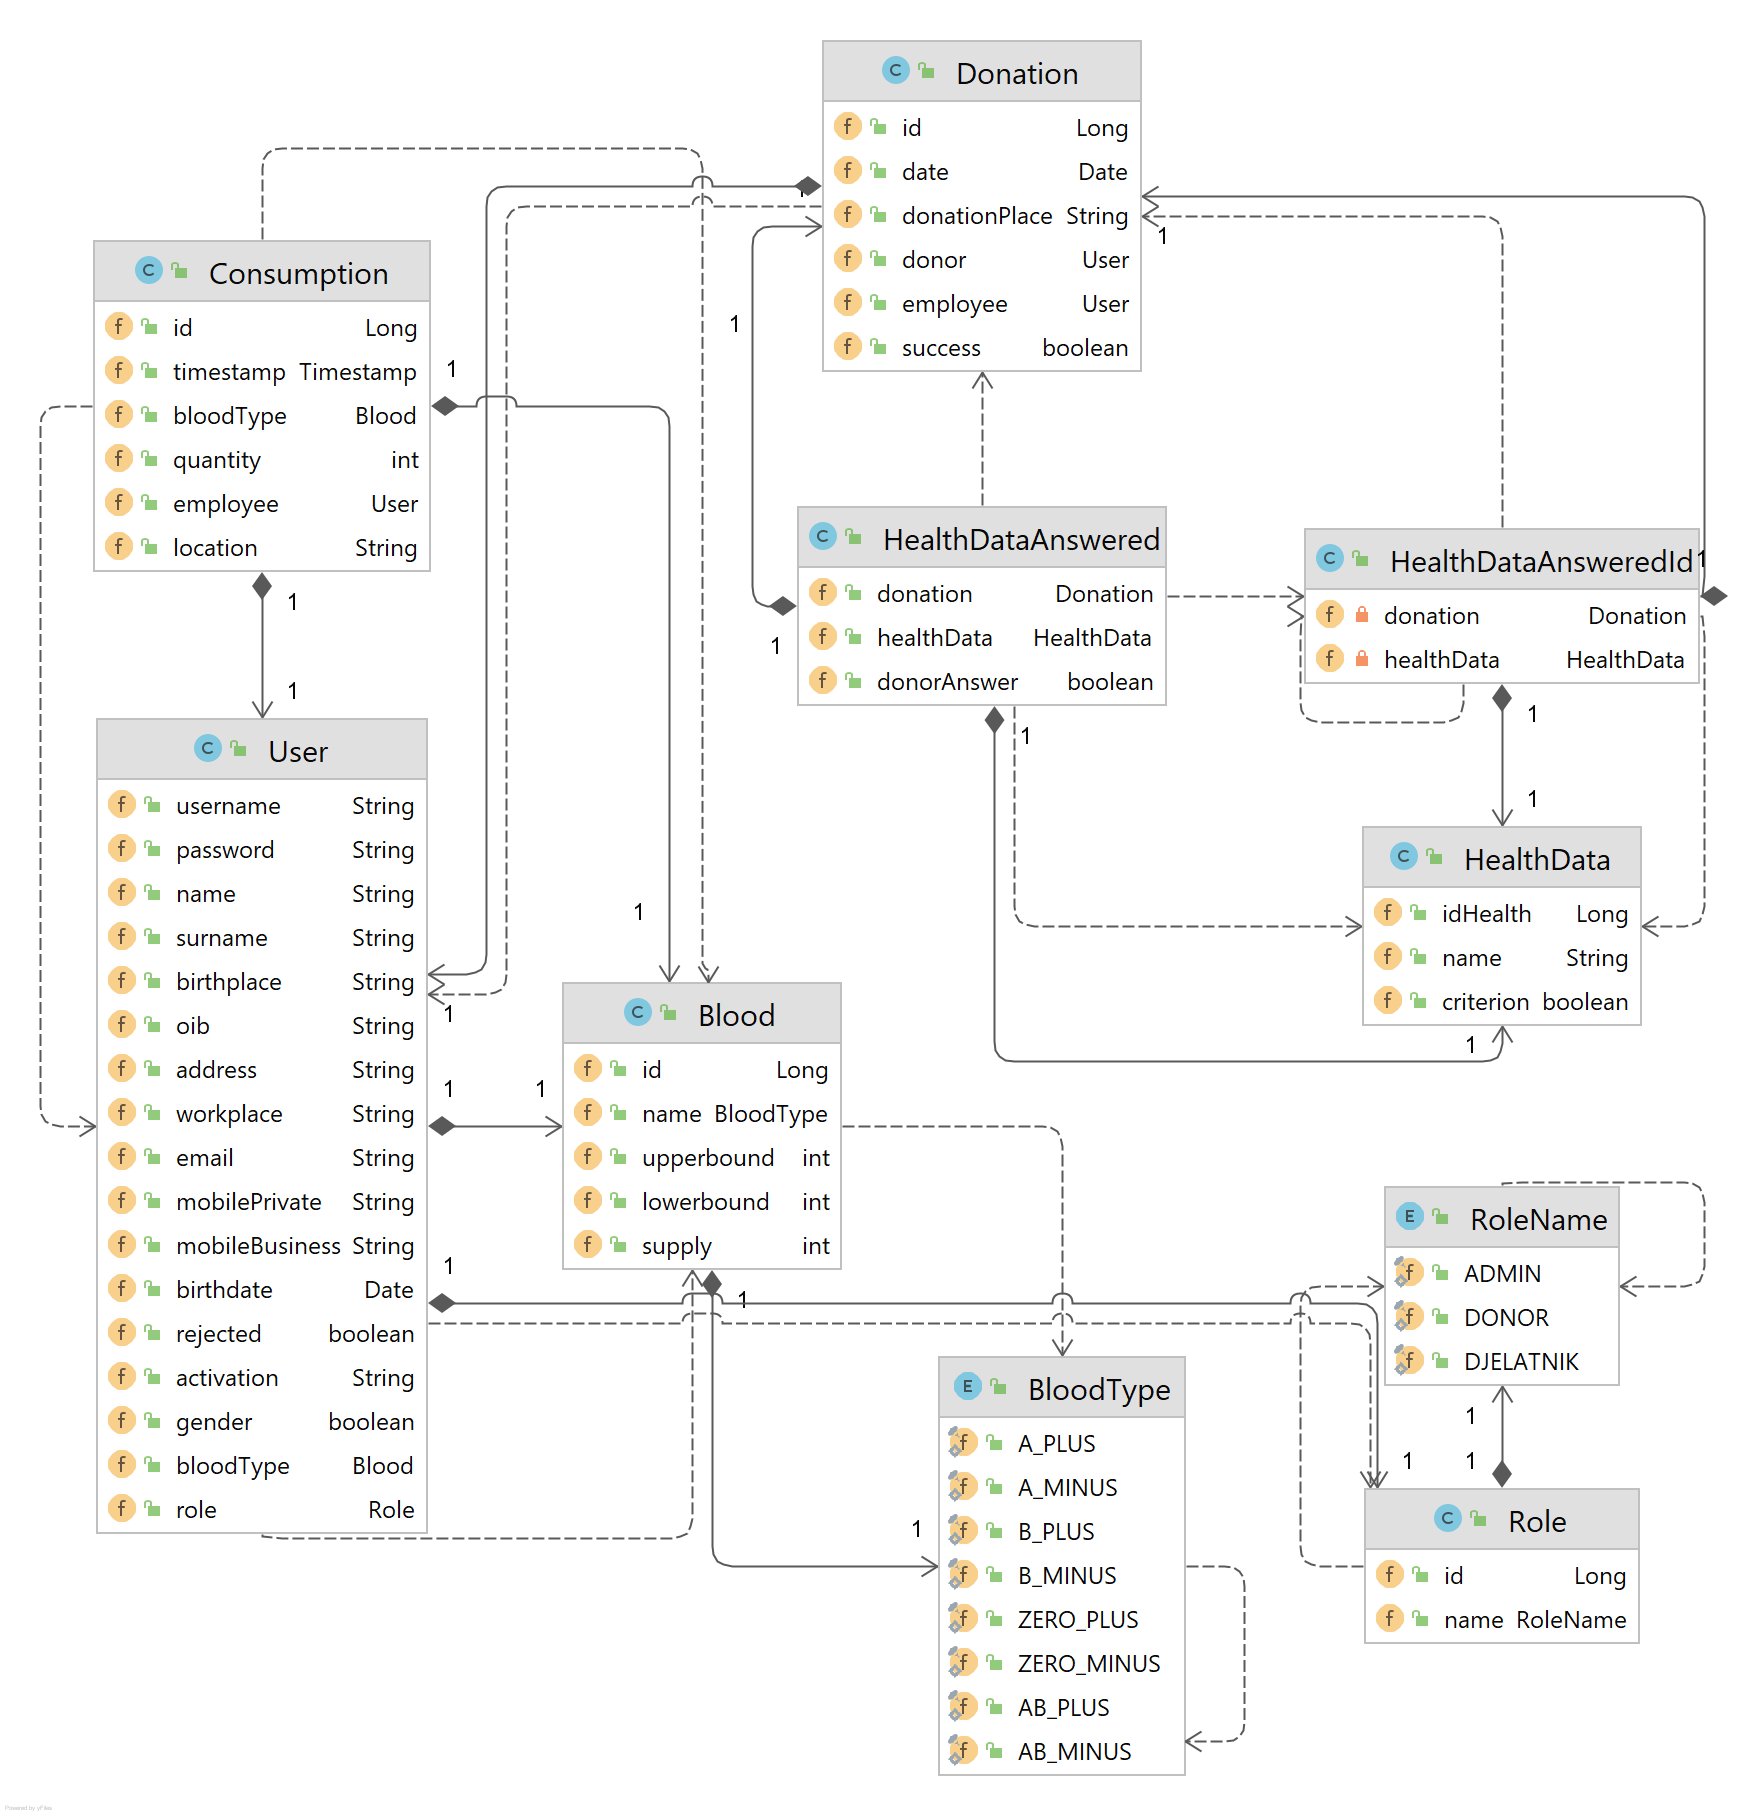
\includegraphics[width=\textwidth, scale=2.0]{dijagrami/dijagram_razreda1}
	\caption{Dijagram razreda koji opisuje model}
	\label{fig:dijagram_modela}
\end{figure}
		
	\eject
<<<<<<< HEAD
	Na idućoj slici prikazana je sloj \textit{backenda} koji je odgovoran za neposrednu komunikaciju s poslužiteljem baze podataka. Kao glavna komponenta na slici prikazano je sučelje JpaRepository, koje predstavlja apstraktni repozitorij podataka. Iz tog sučelja, izvedena su sučelja UserRepository, RoleRepository, BloodRepository, ConsumptionRepository, DonationRepository, HealthDataRepository i HealthDataAnsweredRepository. Ta sučelja predstavljaju repozitorij podataka za prije navedene razrede modela, tj. oni predstavljaju poveznicu s bazom ili DAO (eng. Data Access Object). Također koriste se različite ServiceJpa klase koje koriste te repozitorije, te one implementiraju sučelje imeKlaseService. 
=======
	Na idućoj slici prikazana je sloj \textit{backenda} koji je odgovoran za neposrednu komunikaciju s poslužiteljem baze podataka. Imamo sučelja UserRepository, RoleRepository, BloodRepository, ConsumptionRepository, DonationRepository, HealthDataRepository te HealthDataAnsweredRepository koja predstavljaju apstraktni repozitorij podataka. Ta sučelja predstavljaju repozitorij podataka za prije navedene razrede modela, tj. oni predstavljaju poveznicu s bazom ili DAO (eng. Data Access Object). Također koriste se različite Service klase koje koriste te repozitorije, te one implementiraju sučelje imeKlaseService.  
>>>>>>> devdoc
	
\begin{figure}[H]
	\centering
	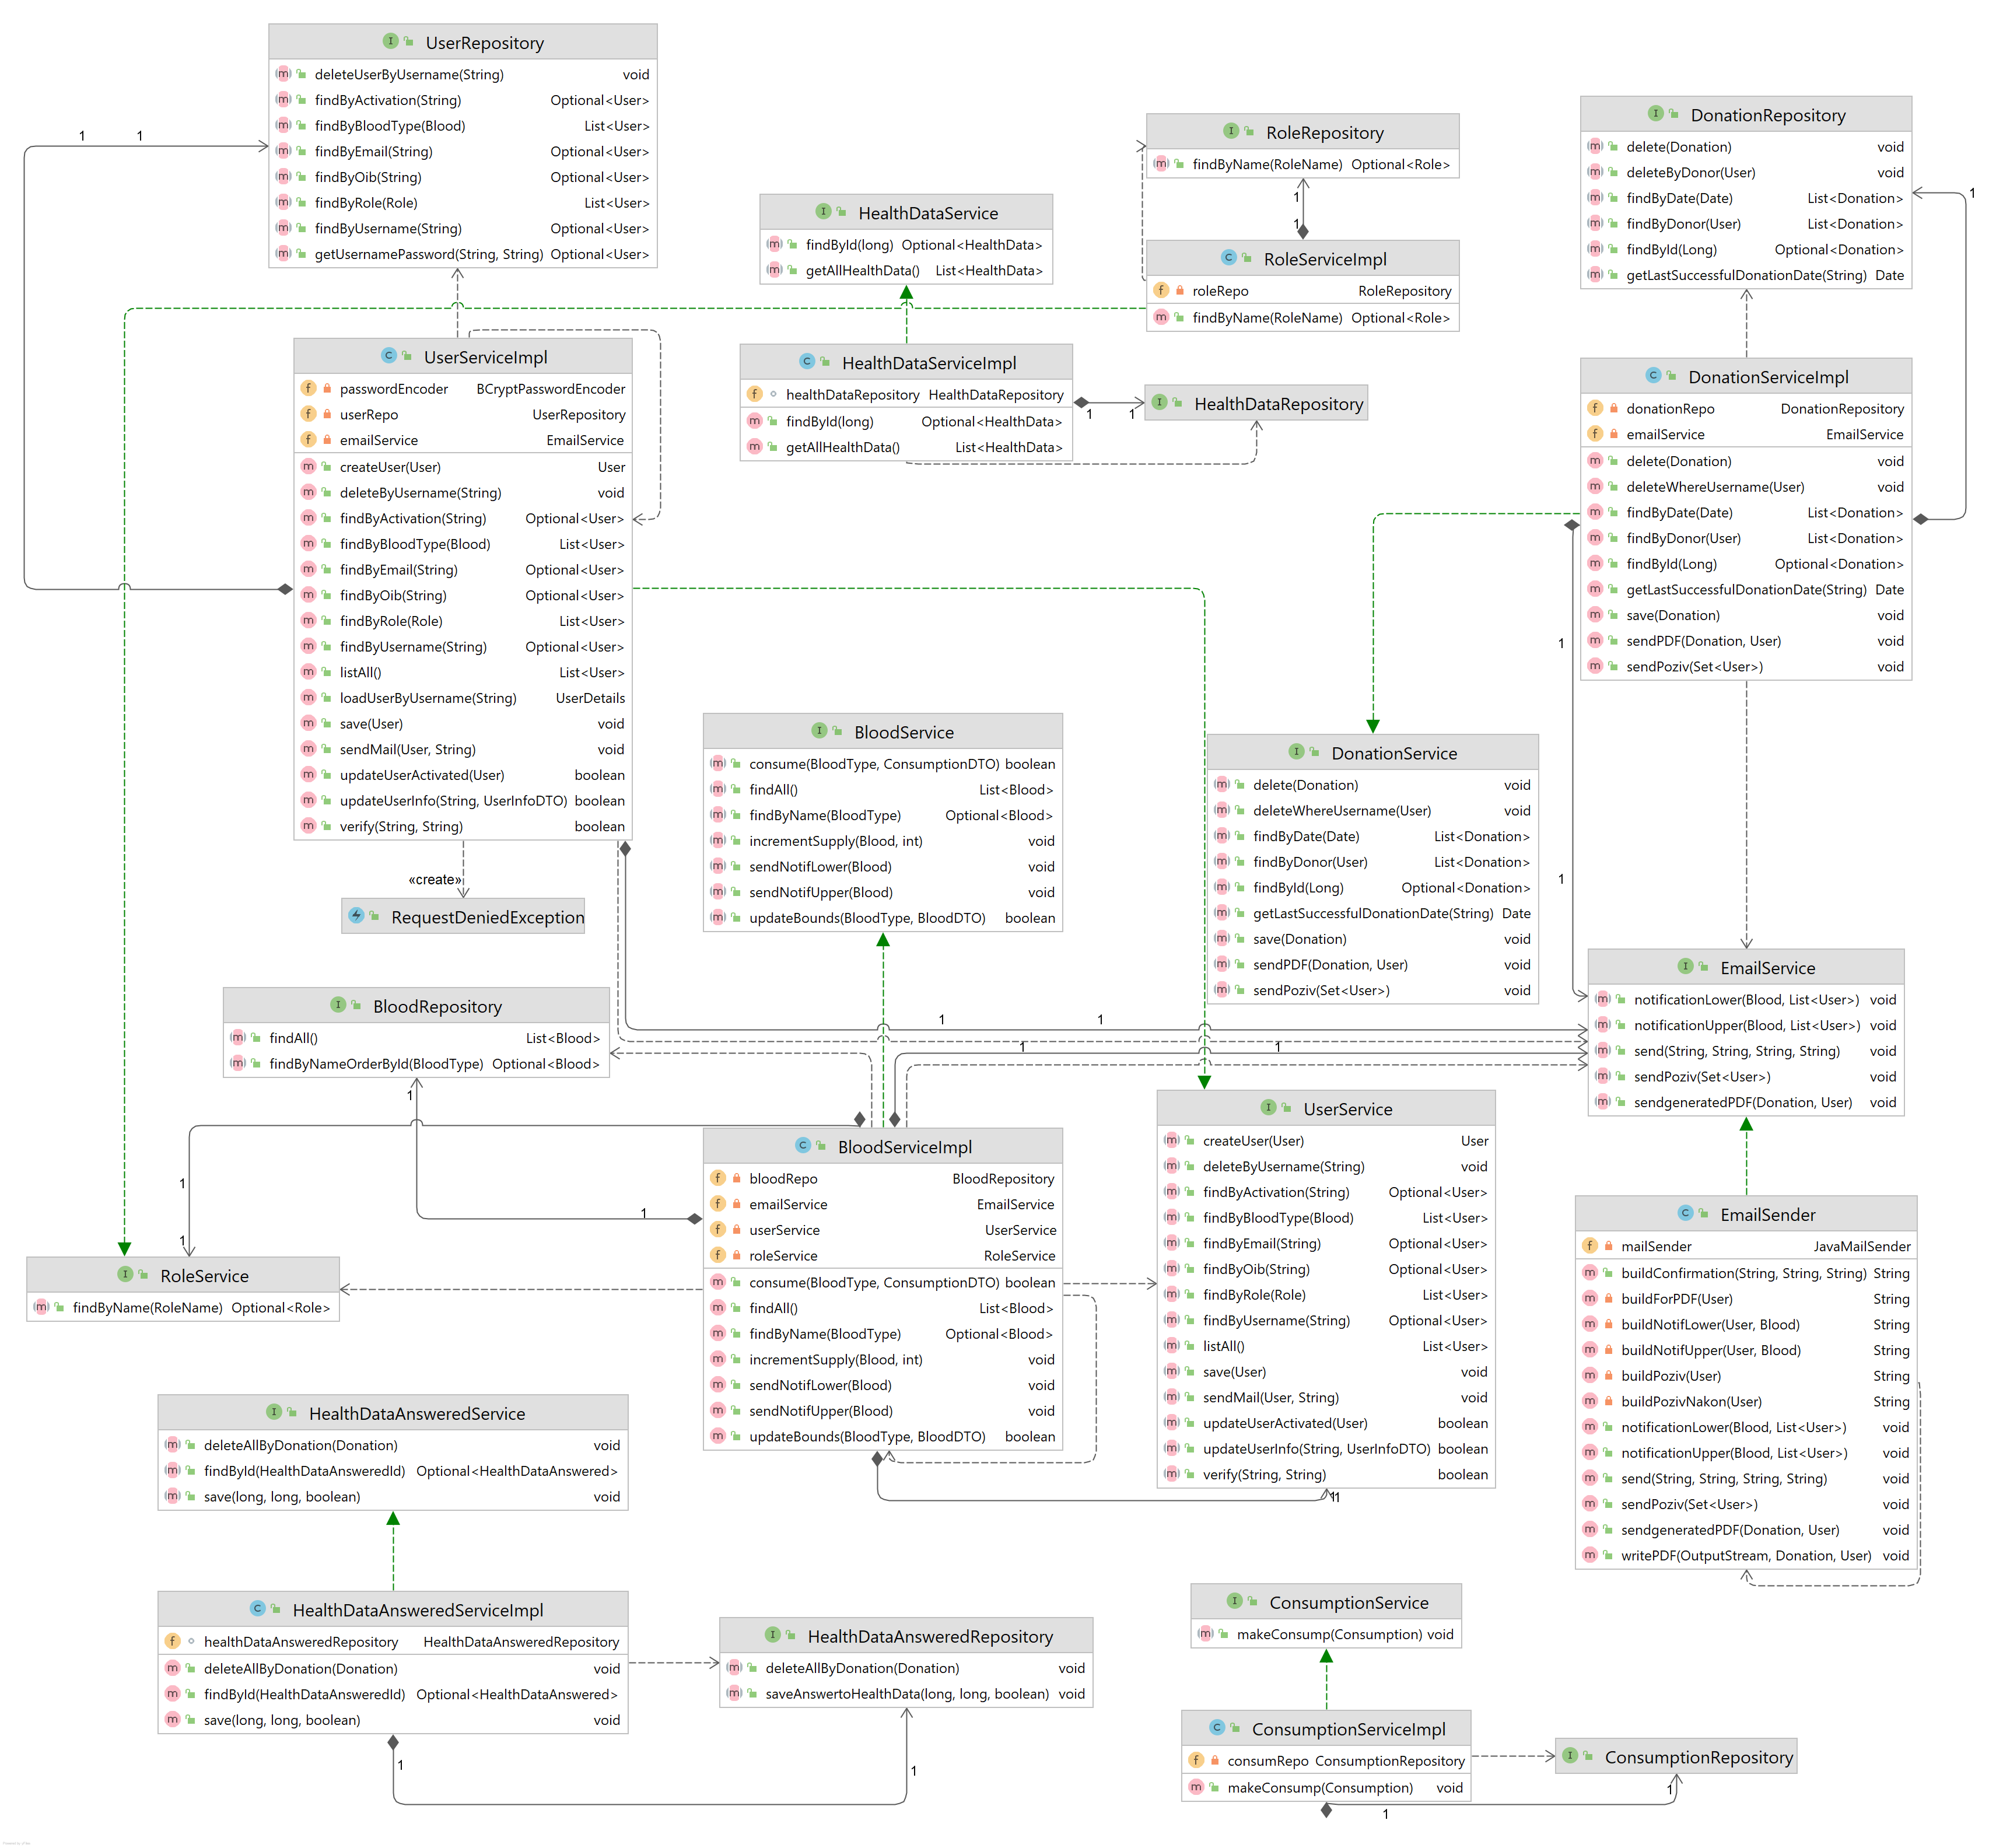
\includegraphics[width=\textwidth, scale=2.0]{dijagrami/dijagram_razreda2}
	\caption{Dijagram razreda koji opisuju repozitorije}
	\label{fig:dijagram_repozitorija}
\end{figure}

\eject

	Na zadnje dvije slike prikazani su \textit{Controlleri} koji komuniciraju s vanjskim svijetom odnosno \textit{frontendom} te upravljaju modelom podataka i DTO-ovi (eng. Data Transfer Object) koje oni koriste za prijenos podataka. Ovdje vidimo razrede UserController, RoleController, BloodController, ConsumptionController, DonationController, AdminController i HealthDataController. Svi ti razredi koriste Java anotaciju RestController koji predstavlja REST endpoint i DTO-ove koji su u paketu \textit{Util}. Ti razredi su oni koji dobivaju zahtjeve iz vanjskog svijeta, a odgovaraju HTTP odgovorima i JSON objektima.

	
\begin{figure}[H]
	\centering
	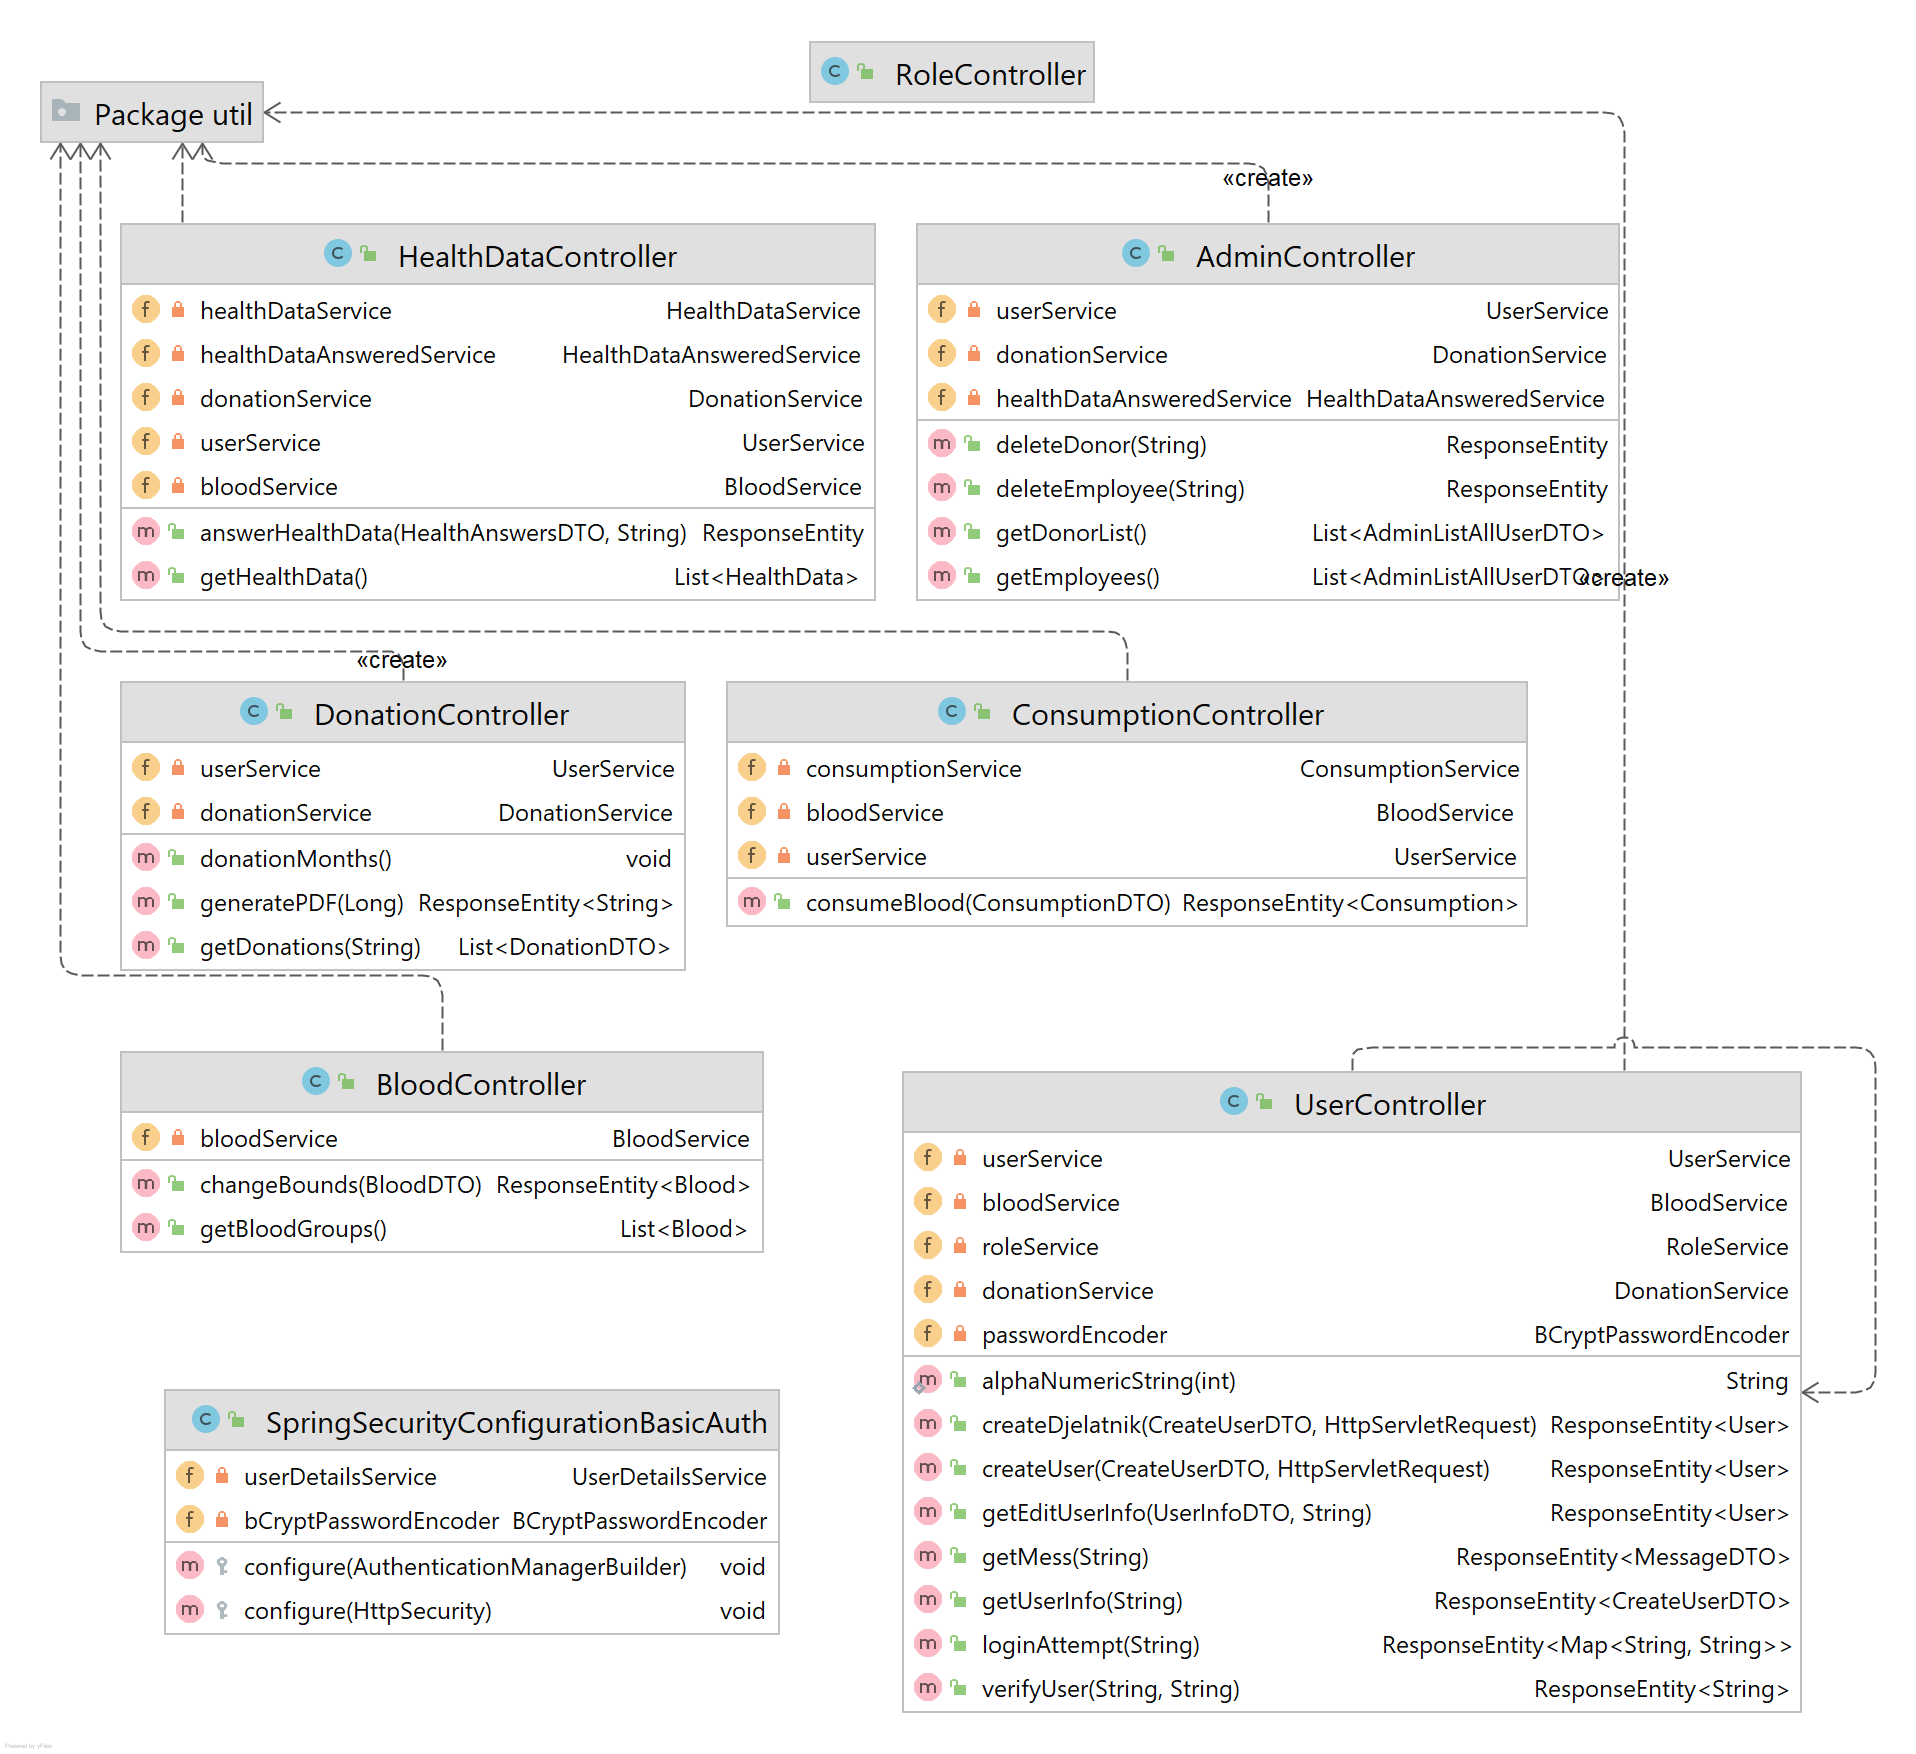
\includegraphics[width=\textwidth, scale=0.5]{dijagrami/dijagram_razreda3}
	\caption{Dijagram razreda koji opisuju kontrolere}
	\label{fig:dijagram_kontrolera}
\end{figure}

\begin{figure}[H]
	\centering
	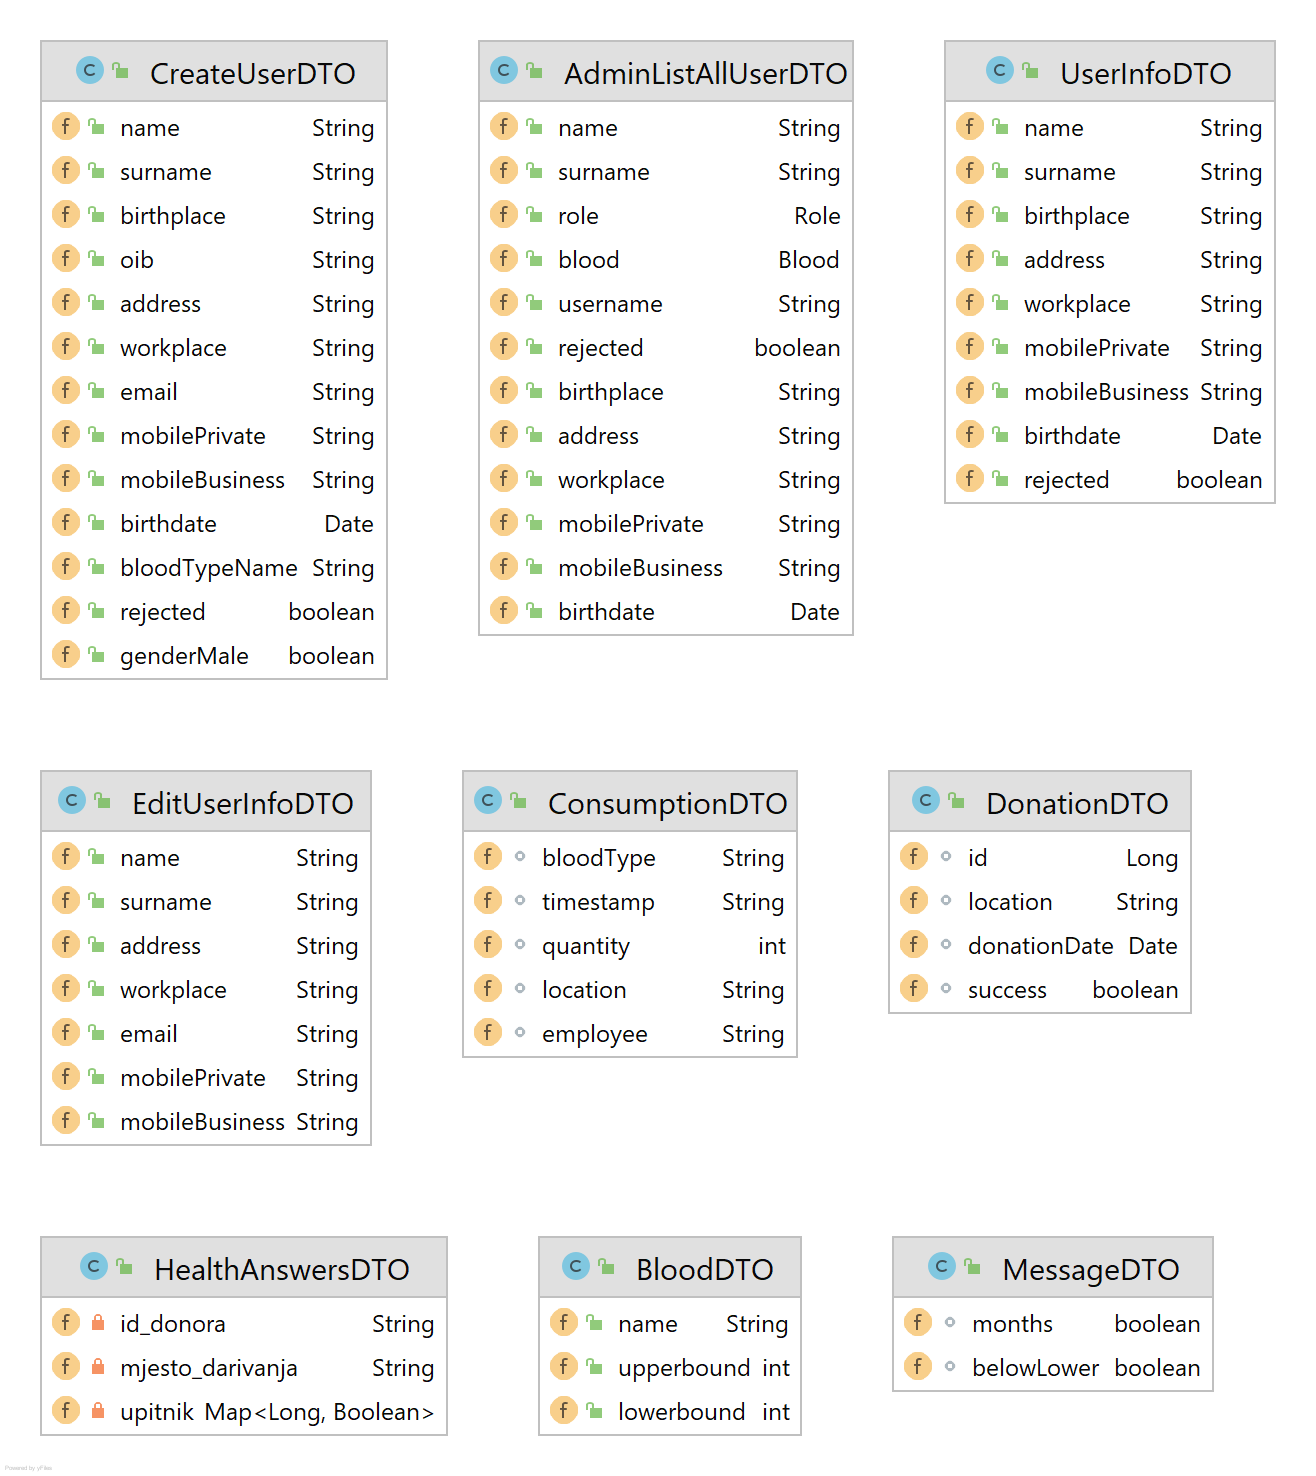
\includegraphics[width=\textwidth, scale=0.5]{dijagrami/dijagram_razreda4}
	\caption{Dijagram razreda koji opisuju DTO-ove}
	\label{fig:dijagram_DTO}
\end{figure}

\eject
			
			
		
		\section{Dijagram stanja}
			Dijagram stanja primijenjuje se za opis stanja objekta i za opisivanje prijelaza iz jednog u drugo stanje. Priložena slika prikazuje stanjadijagram stanja za registriranog donora. Početno stanje je početna stranica aplikacije. U izborniku aplikacije donor može odabrati jednu od mogućnosti. Klikom na "Moji podaci" prikazuju mu se njegovi podaci, koje moeže urediti. Odabirom opcije "Poruke" prikazuju se poruke donoru koje mu javlja sustav. Klikom na 
"Povijest darivanja" prikazuju se prijašnja darivanja za koje, ako je darivanje uspješno,  može izvaditi PDF potvrdu.

\begin{figure}[H]
	\centering
	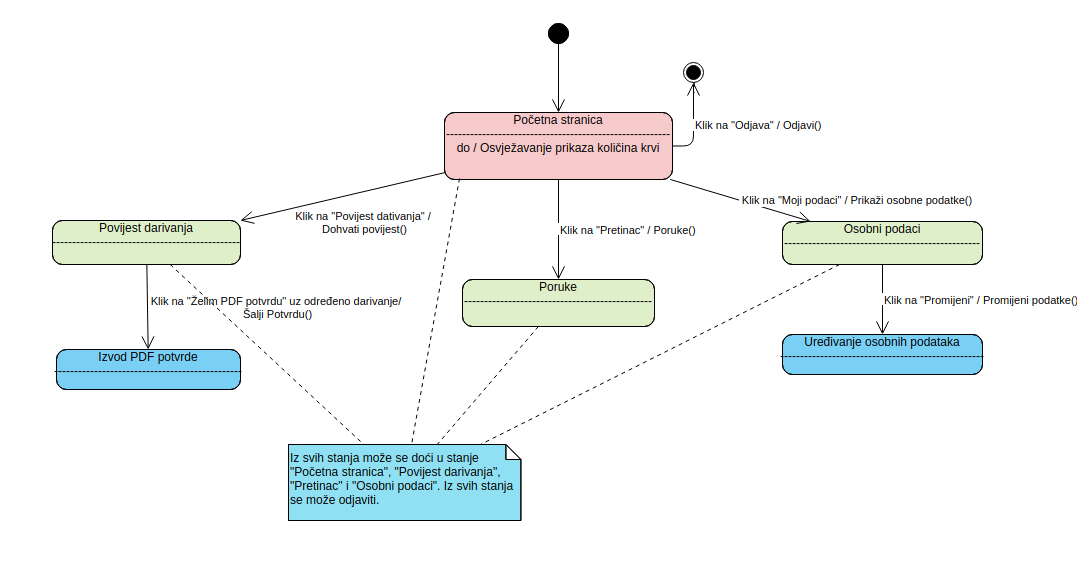
\includegraphics[width=\textwidth, scale=0.7]{dijagrami/dijagram_stanja}
	\caption{Dijagram stanja}
	\label{fig:dijagram_stanja}
\end{figure}
			
			
			
			
			\eject 
		
		\section{Dijagram aktivnosti}
			Dijagram aktivnosti prikazuje povezane aktivnosti na visokoj apstrakcijskoj razini,odnosno intuitivno prikazuje kako podaci teku kroz aplikaciju i kako se
kontrola nad podacima mijenja. U modeliranju toka upravljanja svaki novi korak poduzima se nakon završenog prethodnog. Idući dijagram prikazuje proces smanjivanja količine krvi slanjem u zdravstvenu ustanovu. Ovaj proces može provesti djelatnik banke. Proces započinje prijavom, djelatnik banke odabere krvnu grupu na prikazu količina krvi i unese količinu krvi koju želi poslati zdravstvenoj ustanovi. Kada transakcija završi prikazuje mu se potvrda o smanjenju krvi.
		
\begin{figure}[H]
	\centering
	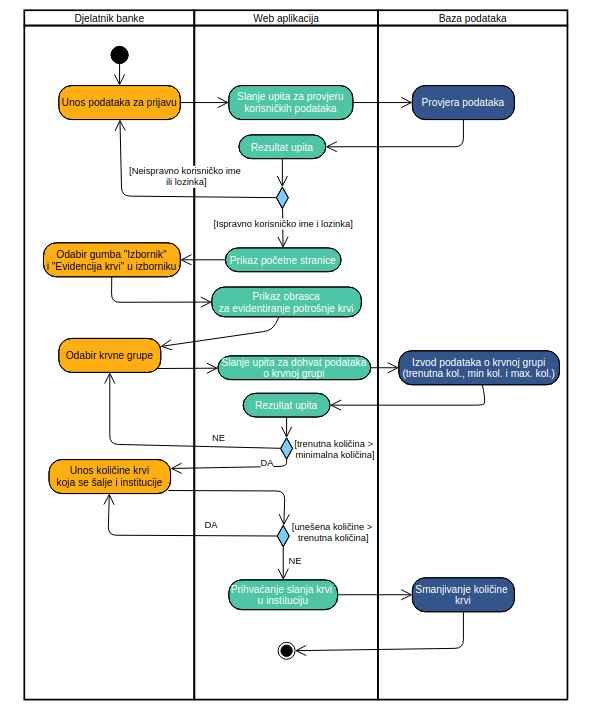
\includegraphics[width=\textwidth, scale=0.5]{dijagrami/dijagram_aktivnosti}
	\caption{Dijagram aktivnosti}
	\label{fig:dijagram_aktivnosti}
\end{figure}
				
			
			\eject
		\section{Dijagram komponenti}
		
			Dijagram komponenti omogućuje nam pogled na sustav s visoke razine apstrak-
cije. Web aplikacija komunicira sa sustavom preko dva sučelja. Prvo sučelje služi
za dohvat samih stranica, dakle HTML, CSS i JS datoteka. Drugo sučelje služi
za komunikaciju između aplikacije i baze podataka. Dakle, web aplikacija šalje
zahtjev REST API-u, koji preko kontrolera komunicira s repozitorijima
podataka, koji predstavljaju sloj povezanosti između baze podataka i kontrolera.  Podaci koji su pristigli
iz baze se šalju dalje MVC arhitekturi u obliku DTO (Data transfer object).
React view komponenta preko dostupnih sučelja komunicira s web aplikacijom te ovisno o korisnikovim akcijama osvježava prikaz i dohvaća nove podatke ili datoteke.

\begin{figure}[H]
	\centering
	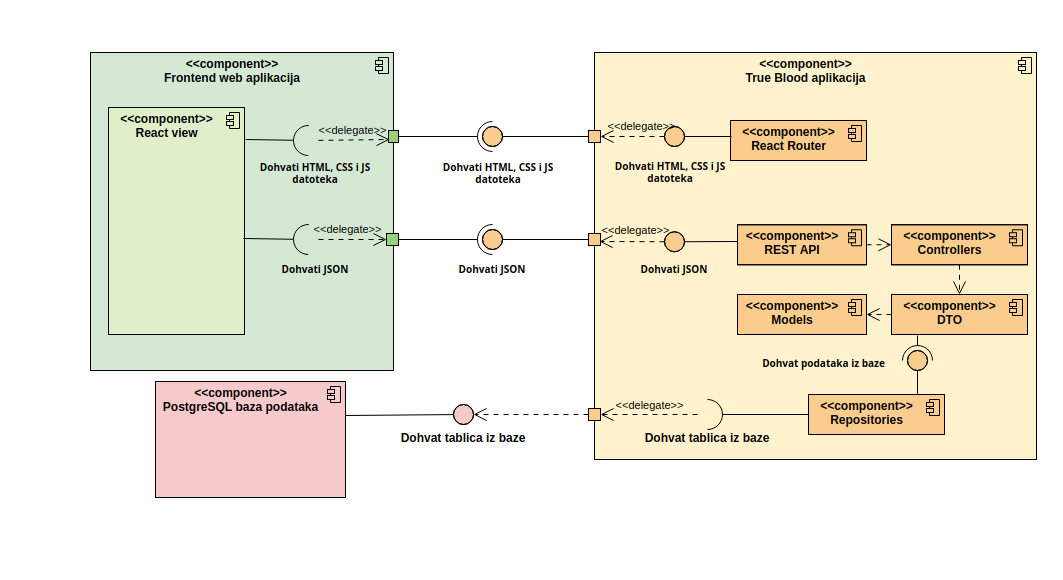
\includegraphics[width=\textwidth, scale=0.5]{dijagrami/dijagram_komponenti}
	\caption{Dijagram komponenti}
	\label{fig:dijagram_komponenti}
\end{figure}
